\documentclass[11pt,a4paper]{article}

\usepackage[utf8]{inputenc}
\usepackage[T1]{fontenc}
\usepackage[brazil]{babel}
\usepackage{lmodern}
\usepackage{microtype}
\usepackage{amsmath}
\usepackage[a4paper,margin=2cm]{geometry}
\usepackage{graphicx}
\usepackage{booktabs}
\usepackage{tabularx}
\usepackage{array}
\usepackage{multirow}
\usepackage{xcolor}
\usepackage{enumitem}
\usepackage{caption}
\usepackage{float}
\usepackage{hyperref}
\hypersetup{colorlinks=true,linkcolor=black,citecolor=black,urlcolor=blue}

% Links para o repositório. \reporef = tag da entrega: os links só funcionam
% depois de \texttt{git push origin entrega3}.
\newcommand{\repobase}{https://github.com/annalujansen/tr2-rdt-unb}
\newcommand{\reporef}{entrega3}
\newcommand{\repodir}[2]{\href{\repobase/tree/\reporef/#1}{#2}}
\newcommand{\repofile}[2]{\href{\repobase/blob/\reporef/#1}{#2}}

\captionsetup{font=small,labelfont=bf}
\setlist{nosep,leftmargin=*}
\setlength{\parskip}{0.4em}
\setlength{\parindent}{0pt}
\renewcommand{\arraystretch}{1.15}

\definecolor{codverde}{HTML}{188038}
\newcommand{\cod}[1]{\textcolor{codverde}{\texttt{\small #1}}}
\newcolumntype{L}{>{\raggedright\arraybackslash}X}
\newcolumntype{R}{>{\raggedleft\arraybackslash}X}
\newcommand{\hd}[1]{\textbf{\begin{tabular}[b]{@{}c@{}}#1\end{tabular}}}

% Marca o que o grupo ainda precisa revisar/completar. Para a versão final:

\title{\vspace{-1.2cm}Relatório Final --- Transferência confiável sobre UDP:\\
de Stop-and-Wait a RTT adaptativo}
\author{%
  CIC0236 -- Teleinformática e Redes 2 -- Turma 01 -- 2026/2 -- Universidade de Brasília\\[0.4em]
  \textbf{Grupo 10} (\cod{-{}-group grupo10})\\
  Anna Luiza Novaes Jansen Silva -- 232024572\\
  Vinicius Henrique Barbosa Silverio de Castro -- 232006832\\[0.4em]
}
\date{}

\begin{document}
\maketitle
\vspace{-0.5cm}

%% ===========================================================================
\section{Introdução e evolução do projeto}

O UDP não garante entrega, ordem nem integridade. O servidor (\cod{137.131.178.229:8080}/UDP) é
\emph{pull-based}: só responde a pedidos (\cod{REQ}), então toda a confiabilidade (detecção de perda,
retransmissão, ordenação e verificação por MD5) tem de existir no cliente. A sessão é sempre a mesma:
\begin{center}
\cod{HELLO} $\rightarrow$ \cod{OK} (tamanho e MD5) $\rightarrow$ \cod{REQ}, \cod{DATA} e \cod{ACK}
por segmento $\rightarrow$ \cod{FIN} (MD5 calculado) $\rightarrow$ \cod{DONE|ok=1}
\end{center}
O projeto evoluiu em três etapas, cada uma motivada por uma limitação medida na anterior.

\subsection{Entrega 1 --- Stop-and-Wait (SAW)}

O primeiro cliente fazia o ciclo mais simples possível: \cod{HELLO}/\cod{OK}, depois, para cada
segmento, \cod{REQ|seq=n}, espera do \cod{DATA} com o mesmo \cod{seq} até o timeout fixo de 500\,ms,
\cod{ACK} e próximo segmento, terminando com \cod{FIN}/\cod{DONE} e conferência do MD5. Duas decisões
de implementação evitaram erros que só apareceriam no MD5: o \cod{DATA} é separado com
\cod{split(b\textquotedbl|\textquotedbl, 3)}, porque o payload é binário e pode conter o byte \cod{|}; e \cod{DATA} com
\cod{seq} diferente do esperado (duplicata atrasada de uma retransmissão) é descartado sem reiniciar
o prazo.

Os três arquivos foram recebidos íntegros (13/10/2026, sem perda simulada):

\begin{table}[H]
\centering\small
\setlength{\tabcolsep}{5pt}
\caption{Entrega 1: SAW com timeout fixo de 500\,ms.}
\label{tab:e1}
\begin{tabular}{@{}l rrrrr@{}}
\toprule
\textbf{Arquivo} & \hd{Tempo\\total} & \hd{RTT\\médio} & \hd{Throughput\\medido} & \hd{Teórico\\($512 \cdot 8/\mathit{RTT}$)} & \hd{Retrans-\\missões}\\
\midrule
small (1\,MB)   & 131,9\,s & 38,49\,ms & 63,62\,kbps & 106,41\,kbps & 105\\
medium (5\,MB)  & 588,7\,s & 39,17\,ms & 71,25\,kbps & 104,56\,kbps & 370\\
large (10\,MB)  & 965,9\,s & 35,58\,ms & 86,84\,kbps & 115,13\,kbps & 465\\
\bottomrule
\end{tabular}
\end{table}

O resultado mais útil da Entrega 1 foi a decomposição do tempo: o tempo total é explicado quase
exatamente por $N \times \mathit{RTT}_{\text{médio}} + \text{retransmissões} \times 0{,}5\,\text{s}$
(a sobra foi de 0,6 a 4,7\,s, menos de 0,5\,\%). Descontando os timeouts, o SAW chega a
104--114\,kbps, o teto de um segmento por RTT. O que afastava o medido do teórico (60\,\% a 75\,\%)
eram as perdas naturais da rede real (2,2\,\% a 4,9\,\% dos envios): cada perda parava o cliente por
500\,ms, cerca de 13 RTTs; no small, 40\,\% do tempo foi espera de timeout. Dois fatos já apontavam
para o que viria depois: a mediana do RTT era de $\sim$26--30\,ms, de modo que o timeout fixo era 17
a 20 vezes maior que o necessário; e o limite de um segmento por RTT pedia mais de um segmento em
trânsito.

\textbf{Resposta ao feedback da Entrega 1.} O professor apontou que a perda de 2,2--4,9\,\% era
alta para um RTT mediano normal ($\sim$26--30\,ms) e perguntou quantos timeouts podem ter sido
prematuros, já que o RTT máximo (473,9\,ms) chegou perto do timeout de 500\,ms.
\begin{itemize}
  \item \textbf{Ambiente:} os três testes rodaram em sequência em 13/10/2026, das 21:15 às 21:44
        (horário de pico do uso doméstico), a partir de Wi-Fi residencial,
        com o cliente atrás de NAT (IP \cod{192.168.100.9}, visto na captura da Seção~\ref{sec:wireshark}).
  \item \textbf{A perda veio do ambiente, não do código:} com o mesmo código e o mesmo timeout de
        500\,ms, o SAW com o arquivo large teve 772 retransmissões (3,6\,\%) às 18:32 de 10/11 e
        apenas 3 (0,015\,\%) às 19:23 do mesmo dia, com o RTT médio caindo de 35,3 para 26,9\,ms.
        A perda natural varia muito com o horário; 13/10 foi um dia ruim.
  \item \textbf{Timeouts prematuros: praticamente nenhum.} Um timeout é prematuro quando o DATA
        original chega depois de 500\,ms. Entre os 31\,873 segmentos entregues sem retransmissão nos
        três arquivos, o RTT passou de 250\,ms em só 12 e de 400\,ms em só 2 (máximo de 473,9\,ms, no
        medium); o percentil 99 ficou em 134--147\,ms. Pela cauda da distribuição, atrasos acima de
        500\,ms seriam no máximo alguns poucos casos entre as 940 retransmissões. Além disso, um DATA
        atrasado que chegasse logo depois do reenvio apareceria no CSV com \cod{rtt\_ms} (medido a
        partir do reenvio) abaixo do RTT mínimo do caminho ($\sim$19\,ms); nos 895 segmentos
        retransmitidos o menor valor foi 19,9\,ms. Os dados indicam que as retransmissões foram,
        quase todas, perdas reais. Na Entrega 3 a captura do Wireshark permitiu medir isso
        diretamente (Seção~\ref{sec:wireshark}).
\end{itemize}

\subsection{Entrega 2 --- Janela deslizante: Go-Back-N (GBN) e Selective Repeat (SR)}\label{sec:e2}

Antes de tudo, o código foi refatorado: o que não depende do protocolo (pacotes, handshake, MD5, CSV,
simulação de perda) foi para \cod{comum.py}, e \cod{saw.py}, \cod{gbn.py} e \cod{sr.py} passaram a
implementar a mesma interface, \cod{run(sess) -> (payloads, rows)}, com o estado em um dicionário
\cod{sess}. Cada protocolo só decide quando enviar \cod{REQ} e o que fazer com cada \cod{DATA}.

As dificuldades principais e como foram resolvidas:
\begin{itemize}
  \item \textbf{Adaptar a janela a um servidor \emph{pull-based}.} No livro, a janela anda com ACKs
        recebidos pelo remetente; aqui o cliente controla tudo e recebe \cod{DATA}. Passamos a tratar
        ``chegou o DATA da base'' como o equivalente do ``chegou o ACK da base''.
  \item \textbf{Simular perda de modo que ela realmente cause retransmissão.} Descartar o ACK
        (abordagem b) não provoca timeout algum neste protocolo, pois o servidor só reage a \cod{REQ}.
        Adotamos a abordagem (a): o \cod{DATA} é descartado com probabilidade $P$ dentro de
        \cod{recv\_data}, antes de qualquer processamento, com \cod{random.Random(seed)} para
        repetibilidade (\cod{-{}-seed 42}) e o mesmo ponto de aplicação nos três protocolos.
  \item \textbf{Separar perda simulada de perda natural.} O CSV ganhou as colunas
        \cod{simulated\_loss}, \cod{sim\_drops} e \cod{recv\_time\_ms}. Uma retransmissão sem perda
        simulada correspondente indica perda natural.
  \item \textbf{Um temporizador por segmento no SR com um único socket.} \cod{recv\_data} espera até o
        menor prazo entre os pendentes (\cod{last\_send[seq] + timeout}), e só os segmentos vencidos
        são reenviados. No GBN há um só temporizador, o da base, e o timeout reenvia a base e todos os
        seguintes.
  \item \textbf{Contar timeouts no GBN.} \cod{timeout\_occurred} marca só o segmento que estava na
        base; o número de eventos precisou ser inferido das retransmissões.
\end{itemize}

Todos os 21 cenários (SAW, GBN e SR $\times$ janelas 4/8/16 $\times$ 0\,\%, 5\,\% e 10\,\%, small,
seed 42) terminaram com o MD5 correto. O resumo dos principais resultados:

\begin{table}[H]
\centering\small
\caption{Entrega 2, arquivo small, timeout fixo: throughput (kbps) / retransmissões / tempo (s).}
\label{tab:e2}
\begin{tabular}{@{}l ccc@{}}
\toprule
\textbf{Protocolo} & \textbf{Sem perda} & \textbf{5\,\% de perda} & \textbf{10\,\% de perda}\\
\midrule
SAW    & 167,2 / 0 / 50,2    & 88,3 / 91 / 95,0      & 52,0 / 220 / 161,3\\
GBN-16 & 2\,025,5 / 0 / 4,1  & 159,5 / 1\,512 / 52,6 & 70,3 / 3\,562 / 119,3\\
SR-16  & 1\,900,7 / 0 / 4,4  & 260,7 / 91 / 32,2     & 153,7 / 220 / 54,6\\
\bottomrule
\end{tabular}
\end{table}

Sem perda, a janela multiplica a vazão ($\sim$12$\times$ com $N = 16$) e GBN e SR são equivalentes.
Com perda, o quadro muda: o GBN reenvia a janela inteira a cada timeout (3\,562 retransmissões contra
220 do SR com 10\,\%, cerca de 16$\times$) e seus timeouts de 500\,ms se somam, enquanto no SR eles se
sobrepõem (220 timeouts, mas só 98 paradas de mais de 300\,ms). Uma varredura extra do tamanho da
janela, sem perda, mostrou que a vazão estabiliza em $\sim$2\,700--2\,900\,kbps a partir de
$N \approx 32$--48, e que em $N = 128$ surgem perdas naturais que derrubam o GBN para
$\sim$1\,700\,kbps. Uma lição de método: a rede varia de um dia para o outro (o SAW sem perda deu
167\,kbps na Entrega 2 contra 64\,kbps na Entrega 1, com RTT médio de $\sim$24\,ms contra
$\sim$38\,ms). Por isso, comparações só são válidas entre execuções feitas nas mesmas condições, e é o
que fazemos na Entrega 3.

O custo dominante com perda continuava sendo o timeout fixo: no SR-16 com 10\,\%, cada uma das 220
perdas custava 500\,ms de espera, para um RTT típico de $\sim$25--35\,ms.

\subsection{Entrega 3 --- RTT adaptativo}

A Entrega 3 ataca exatamente esse custo: em vez de esperar 500\,ms, o cliente estima o RTT por EWMA e
usa $\mathit{RTT}_{est} + 4 \times \mathit{DevRTT}$ como timeout, aplicado a GBN e SR (o SAW permanece
com timeout fixo, como referência). As dificuldades foram: (i) o RTT medido de um segmento
retransmitido é ambíguo, o que já havia sido antecipado na Entrega 1 e foi resolvido com o algoritmo
de Karn; (ii) o timeout agora muda ao longo da execução, então o prazo de cada \cod{REQ} precisa ser
guardado no momento do envio (\cod{timeout\_at\_send}), tanto para o temporizador individual do SR
quanto para o temporizador único da base no GBN; e (iii) para saber se um timeout foi necessário ou
desnecessário, passamos a estimar as retransmissões espúrias (retransmissões menos DATA descartados
pela simulação). A evolução, em resumo:

\begin{table}[H]
\centering\small
\caption{Evolução do projeto.}
\label{tab:evolucao}
\begin{tabularx}{\textwidth}{@{}c L L L@{}}
\toprule
\textbf{Entrega} & \textbf{Implementação} & \textbf{Limitação medida} & \textbf{O que motivou a seguinte}\\
\midrule
1 & SAW, timeout fixo & 1 segmento por RTT ($\sim$105--115\,kbps de teto); perdas custam 500\,ms & Mais segmentos em trânsito\\
2 & GBN e SR, perda simulada & Com perda, GBN reenvia a janela toda; SR ainda espera 500\,ms por perda & Timeout proporcional ao RTT real\\
3 & Timeout adaptativo (EWMA + Karn) & Seções~\ref{sec:rtt} e~\ref{sec:comparacao} & ---\\
\bottomrule
\end{tabularx}
\end{table}

%% ===========================================================================
\section{RTT adaptativo --- implementação}\label{sec:rtt}

\subsection{Fórmulas e regras implementadas}

O estimador está em \cod{update\_rtt\_estimator} (\cod{comum.py}) e roda quando um segmento é aceito,
com $R$ = \cod{rtt\_ms} = instante de chegada do \cod{DATA} $-$ instante do último \cod{REQ} daquele
segmento:
\begin{align*}
\mathit{DevRTT} &= (1-\beta)\,\mathit{DevRTT} + \beta\,\lvert R - \mathit{RTT}_{est}\rvert\\
\mathit{RTT}_{est} &= (1-\alpha)\,\mathit{RTT}_{est} + \alpha\,R\\
\mathit{RTO} &= \mathit{RTT}_{est} + 4\,\mathit{DevRTT}
\end{align*}
\begin{itemize}
  \item \textbf{Inicialização} (primeira amostra válida, como no TCP): $\mathit{RTT}_{est} = R$ e
        $\mathit{DevRTT} = R/2$. Até essa primeira amostra o timeout é o valor de \cod{-{}-timeout} (500\,ms).
  \item \textbf{Desvio:} calculado com o $\mathit{RTT}_{est}$ anterior à atualização, como no enunciado.
  \item \textbf{Timeout:} limitado a [\cod{-{}-min-rto} = 1\,ms, 60\,s] apenas para evitar RTO zero ou
        espera ilimitada.
  \item \textbf{Karn:} só amostras de segmentos sem retransmissão atualizam o estimador
        (\cod{retransmissions == 0}), pois, após um reenvio, o \cod{DATA} recebido pode ser resposta ao
        \cod{REQ} original e o RTT medido a partir do último envio ficaria artificialmente curto. Pela
        mesma razão, o RTT médio dos resumos também usa só amostras Karn-válidas.
  \item \textbf{RTO guardado por envio:} \cod{send\_req} registra \cod{timeout\_at\_send[seq]}. No SR,
        o prazo de cada segmento é \cod{last\_send[seq] + timeout\_at\_send[seq]}; no GBN, o
        temporizador único da base usa o RTO guardado no envio da base e é reiniciado quando a base
        avança ou é retransmitida. O \cod{timeout\_ms} do CSV é, portanto, o RTO vigente no envio do
        último \cod{REQ} do segmento.
\end{itemize}

O CSV por segmento registra \cod{rtt\_ms}, \cod{rtt\_estimated\_ms}, \cod{dev\_rtt\_ms},
\cod{timeout\_ms}, \cod{timeout\_mode}, \cod{alpha} e \cod{beta}. Uma limitação assumida: não
implementamos o \emph{backoff} exponencial do TCP (dobrar o RTO após cada timeout); com perdas
independentes e RTT estável isso não foi necessário, mas seria o primeiro ajuste em um caminho com
congestionamento real.

Um ponto específico deste ambiente: com janela 16 o RTT medido inclui o enfileiramento dos \cod{REQ}
em voo (na Entrega 2, o RTT médio subiu de $\sim$24\,ms para $\sim$32--34\,ms com $N = 16$). O
estimador mede esse RTT efetivo, que é justamente o que importa para decidir quando um \cod{DATA}
está atrasado.

\subsection{Escolha de \texorpdfstring{$\alpha$}{alfa} e \texorpdfstring{$\beta$}{beta}}\label{sec:alfa-beta}

Os valores do TCP ($\alpha = 0{,}125$ e $\beta = 0{,}25$) foram pensados para a Internet em geral.
Para decidir o que funciona melhor neste ambiente (RTT $\sim$22--35\,ms, mediana $\sim$26--30\,ms e
picos de até $\sim$470\,ms observados na Entrega 1), fizemos uma varredura $\alpha \times \beta$ com
SR-16 e o arquivo small, em três níveis de perda simulada, com repetições e médias por combinação.
Para cada combinação foram comparados:
\begin{itemize}
  \item \textbf{throughput médio} (kbps), que resume o custo total das esperas;
  \item \textbf{retransmissões espúrias} = retransmissões $-$ DATA descartados pela simulação. No SR
        cada descarte exige exatamente 1 retransmissão, então o excedente é timeout que estourou com o
        DATA ainda a caminho; esta é a medida do risco de um timeout agressivo demais;
  \item \textbf{timeout médio} (ms), que mostra quão folgado ou apertado o RTO ficou.
\end{itemize}
O esperado era um compromisso: $\alpha$ e $\beta$ maiores acompanham mais rápido as variações do RTT,
mas deixam o RTO mais nervoso; $\beta$ menor aperta o RTO e reduz a espera por perda, mas aumenta o
risco de timeout espúrio quando o RTT tem picos.

\begin{table}[H]
\centering\small
\caption{Varredura $\alpha \times \beta$: SR-16, arquivo small, média de 2 execuções por combinação.
Vazão em kbps; espúrias = retransmissões $-$ DATA descartados, com perda de 0 / 5 / 10\,\%.}
\label{tab:varredura}
\begin{tabular}{@{}ll rrrr c@{}}
\toprule
$\alpha$ & $\beta$ & \textbf{0\,\%} & \textbf{5\,\%} & \textbf{10\,\%} & \textbf{Média} & \textbf{Espúrias (0 / 5 / 10\,\%)}\\
\midrule
0,0625 & 0,125 & 923,0    & 1\,198,4 & 991,2    & 1\,037,5 & 2\,845 / 920 / 700\\
0,0625 & 0,25  & 1\,248,0 & 1\,159,0 & 955,6    & 1\,120,9 & 1\,707 / 779 / 756\\
0,0625 & 0,5   & 1\,006,6 & 1\,078,6 & 917,6    & 1\,000,9 & 3\,590 / 1\,388 / 707\\
0,125  & 0,125 & 1\,040,3 & 1\,177,6 & 959,9    & 1\,059,3 & 2\,465 / 942 / 830\\
0,125 (TCP) & 0,25 (TCP) & 1\,466,9 & 1\,156,8 & 940,6 & 1\,188,1 & 1\,906 / 1\,128 / 904\\
0,125  & 0,5   & 1\,544,5 & 1\,136,0 & 986,8    & 1\,222,4 & 1\,202 / 1\,182 / 1\,006\\
\textbf{0,25} & \textbf{0,125} & \textbf{1\,564,6} & 1\,176,3 & \textbf{1\,050,4} & \textbf{1\,263,8} & 1\,408 / 1\,154 / 930\\
0,25   & 0,25  & 1\,528,5 & 1\,120,8 & 820,8    & 1\,156,7 & 1\,596 / 1\,524 / 1\,942\\
0,25   & 0,5   & 1\,484,9 & 1\,210,7 & 836,7    & 1\,177,4 & 1\,723 / 1\,356 / 2\,124\\
0,5    & 0,125 & 1\,505,1 & 1\,114,6 & 825,6    & 1\,148,4 & 1\,863 / 2\,035 / 3\,192\\
0,5    & 0,25  & 1\,417,9 & 1\,174,5 & 872,9    & 1\,155,1 & 1\,834 / 1\,761 / 2\,682\\
0,5    & 0,5   & 1\,489,3 & 1\,171,5 & 932,4    & 1\,197,7 & 1\,872 / 1\,768 / 1\,555\\
\bottomrule
\end{tabular}
\end{table}

\textbf{Escolha: $\alpha = 0{,}25$ e $\beta = 0{,}125$.} Essa combinação teve a maior vazão média nas
três perdas (1\,263,8\,kbps), 6\,\% acima da dos valores do TCP ($\alpha = 0{,}125$ e $\beta = 0{,}25$:
1\,188,1\,kbps), e foi a melhor com 0\,\% (1\,564,6\,kbps) e com 10\,\% de perda (1\,050,4\,kbps). Com
5\,\% as combinações ficam próximas (1\,079 a 1\,211\,kbps), dentro do que duas repetições por ponto
permitem distinguir; por isso a escolha se apoia no conjunto das três perdas, não em um ponto isolado.

Dois efeitos aparecem nos dados (Figura~\ref{fig:varredura}). Primeiro, $\alpha$ maior aproxima o RTO
do RTT: com 10\,\% de perda, o timeout médio cai de 41--44,5\,ms ($\alpha = 0{,}0625$) para
32--36,5\,ms ($\alpha = 0{,}5$). Segundo, aproximar demais o RTO tem preço: $\alpha = 0{,}5$ com
10\,\% de perda deu as piores vazões (826--932\,kbps) e até 3\,750 retransmissões (3\,192 espúrias com
$\beta = 0{,}125$). No outro extremo, $\alpha = 0{,}0625$ reage devagar e ficou abaixo de
1\,250\,kbps com 0\,\% de perda, contra 1\,418--1\,565\,kbps para $\alpha \geq 0{,}25$, embora tenha
poucas espúrias com 10\,\%.

Os valores do TCP ficaram a 6\,\% do melhor neste ambiente, então o ganho de ajustar $\alpha$ e
$\beta$ é pequeno perto do ganho do adaptativo sobre o fixo (Seção~\ref{sec:comparacao}) e incerto
com duas repetições. Todas as combinações tiveram muitas retransmissões espúrias, inclusive com 0\,\%
de perda (1\,202 a 3\,590 retransmissões para 2\,048 segmentos), tema da Seção~\ref{sec:fixo-basta}.

\begin{figure}[H]
  \centering
  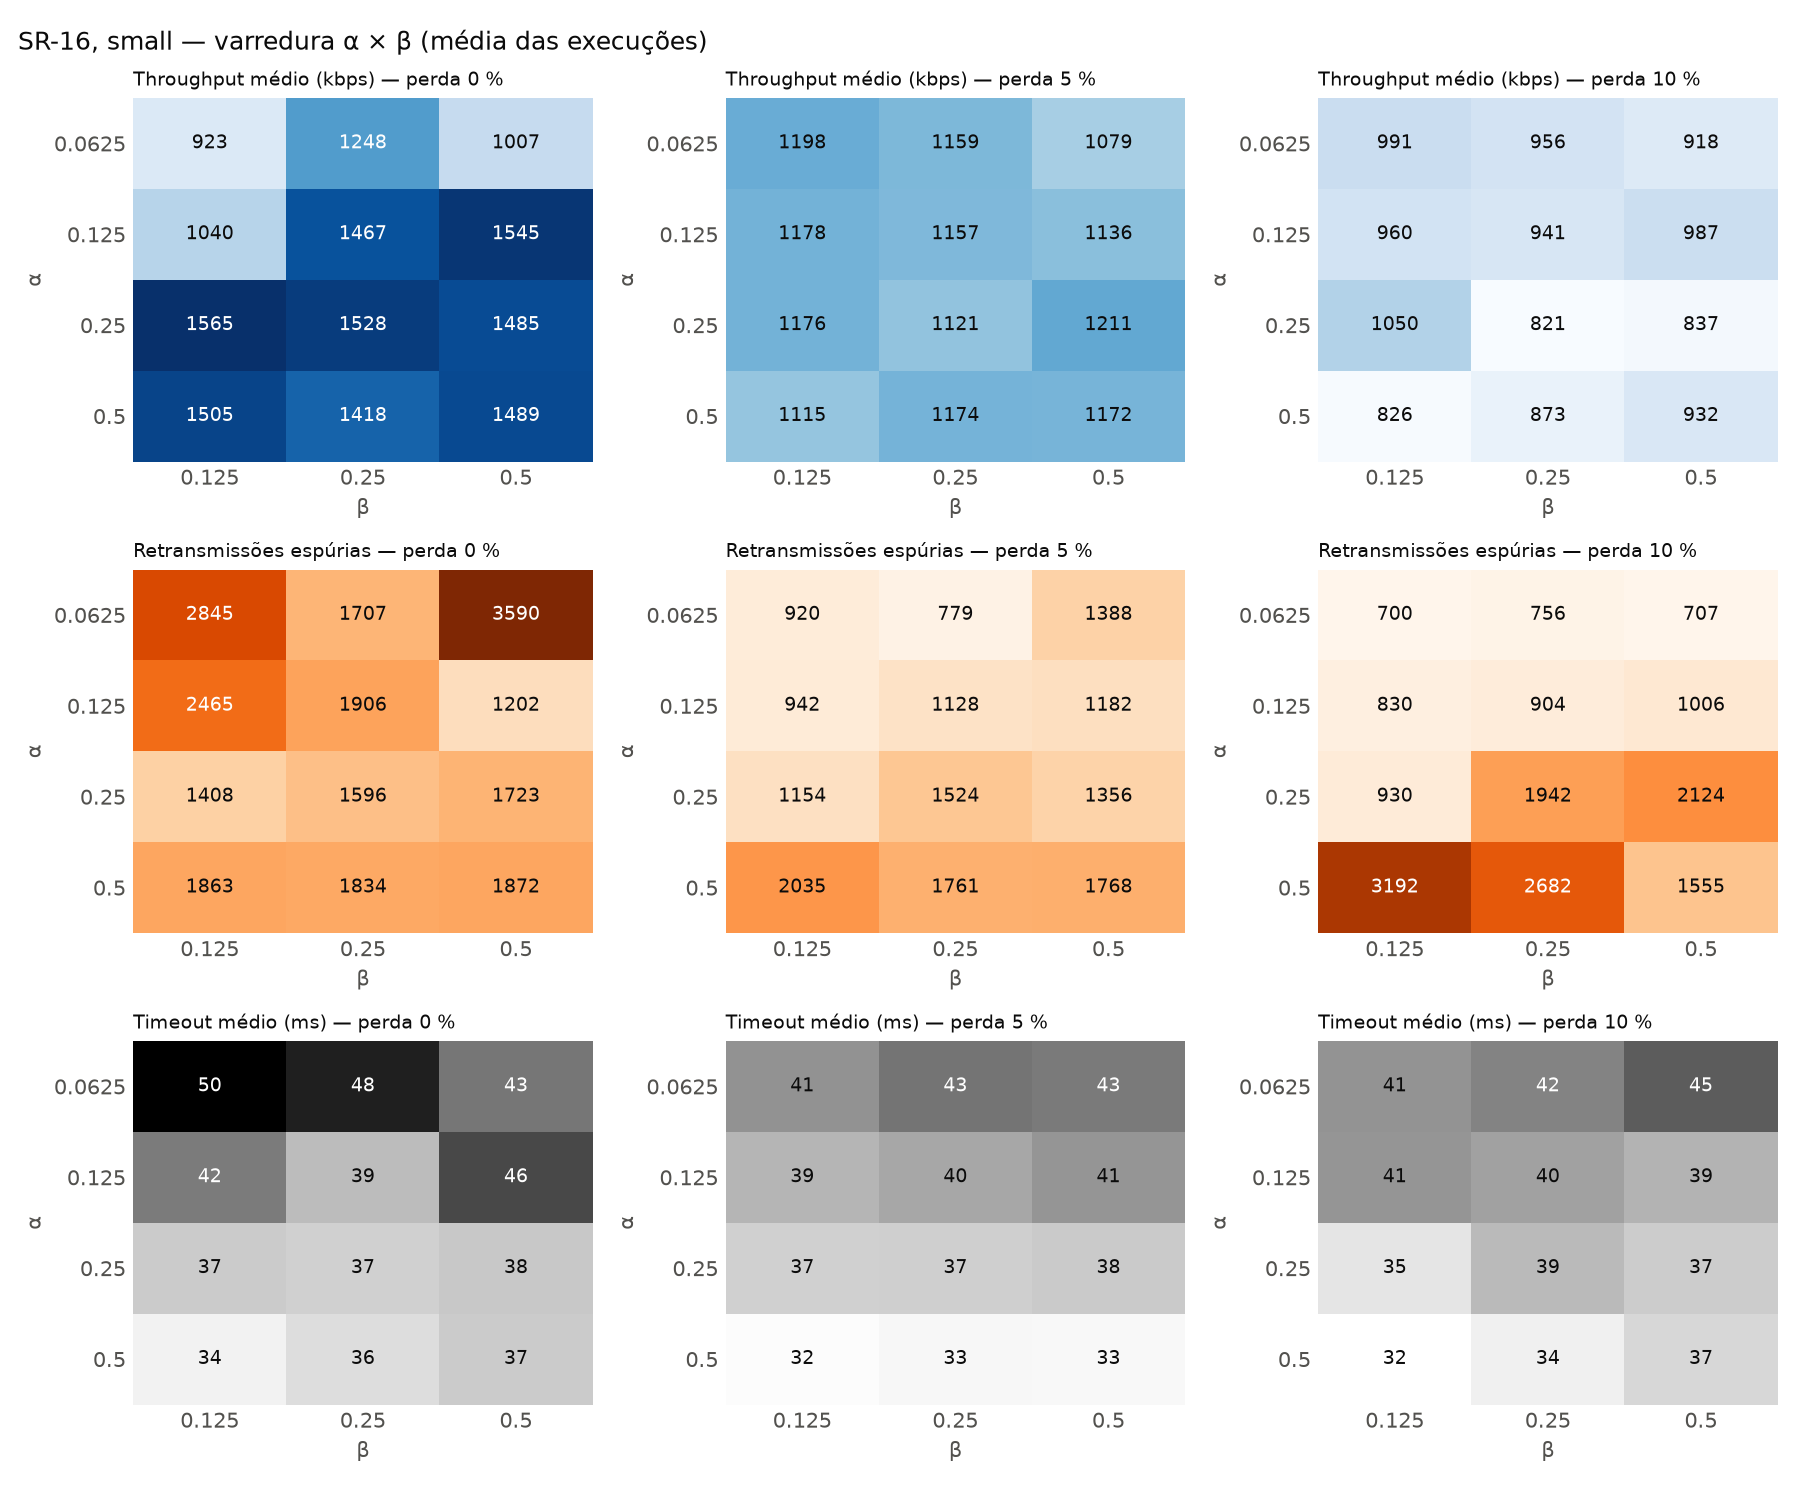
\includegraphics[width=0.92\textwidth]{figuras/varredura_alfa_beta.png}
  \caption{Mapa de calor da varredura $\alpha \times \beta$: throughput, retransmissões espúrias e
  timeout médio por perda simulada.}
  \label{fig:varredura}
\end{figure}

\subsection{Convergência do estimador e evolução do timeout}\label{sec:conv}

As Figuras~\ref{fig:rtt} e~\ref{fig:rtt-zoom} mostram os dois gráficos pedidos, com
$\alpha = 0{,}25$ e $\beta = 0{,}125$, para o SR-16 adaptativo com o arquivo large (20\,480 segmentos,
sem perda simulada; a mesma execução capturada no Wireshark, Seção~\ref{sec:wireshark}). Em cada
figura, o \textbf{painel de cima} é o RTT estimado $\times$ RTT medido por segmento e o
\textbf{painel de baixo} é o timeout ao longo da transferência.

\textbf{Convergência (Figura~\ref{fig:rtt-zoom}).} Os 16 primeiros \cod{REQ} saem com o timeout
inicial de 500\,ms. Quando chega o primeiro \cod{DATA}, o estimador começa em
$\mathit{RTT}_{est} = 24{,}0$\,ms e $\mathit{DevRTT} = 12{,}0$\,ms ($R/2$), e o timeout cai para
72\,ms no segmento 16 e para $\sim$31\,ms no segmento 40. A partir daí o $\mathit{DevRTT}$ continua
diminuindo e o $\mathit{RTT}_{est}$ acompanha os degraus do RTT medido (21--28\,ms), que mudam quando
o enfileiramento dos 16 \cod{REQ} em voo muda. Com $\alpha = 0{,}25$ cada degrau é absorvido em
poucas amostras.

\textbf{Adaptação do timeout (Figura~\ref{fig:rtt}).} Ao longo da transferência, o timeout segue o
RTT estimado com folga de só 3--6\,ms, porque o $\mathit{DevRTT}$ fica em torno de 1\,ms (0,9\,ms no
fim). Quando o RTT sobe num degrau, o timeout sobe junto; quando cai, o timeout cai. É o comportamento
esperado do estimador, mas tem um efeito colateral visível nos dois painéis: as marcas pretas (10\,176
segmentos com timeout) e os X laranja (RTT de segmentos retransmitidos, quase todos abaixo de 20\,ms, medidos
a partir do reenvio e ignorados pelo algoritmo de Karn). Cada pico de RTT acima da folga dispara
timeouts em sequência, e como essas amostras longas são justamente as descartadas por Karn, o
estimador não ``aprende'' com elas e o RTO continua apertado. As consequências estão na
Seção~\ref{sec:fixo-basta}, e a correção, na Seção~\ref{sec:rto-min}.

\begin{figure}[!htbp]
  \centering
  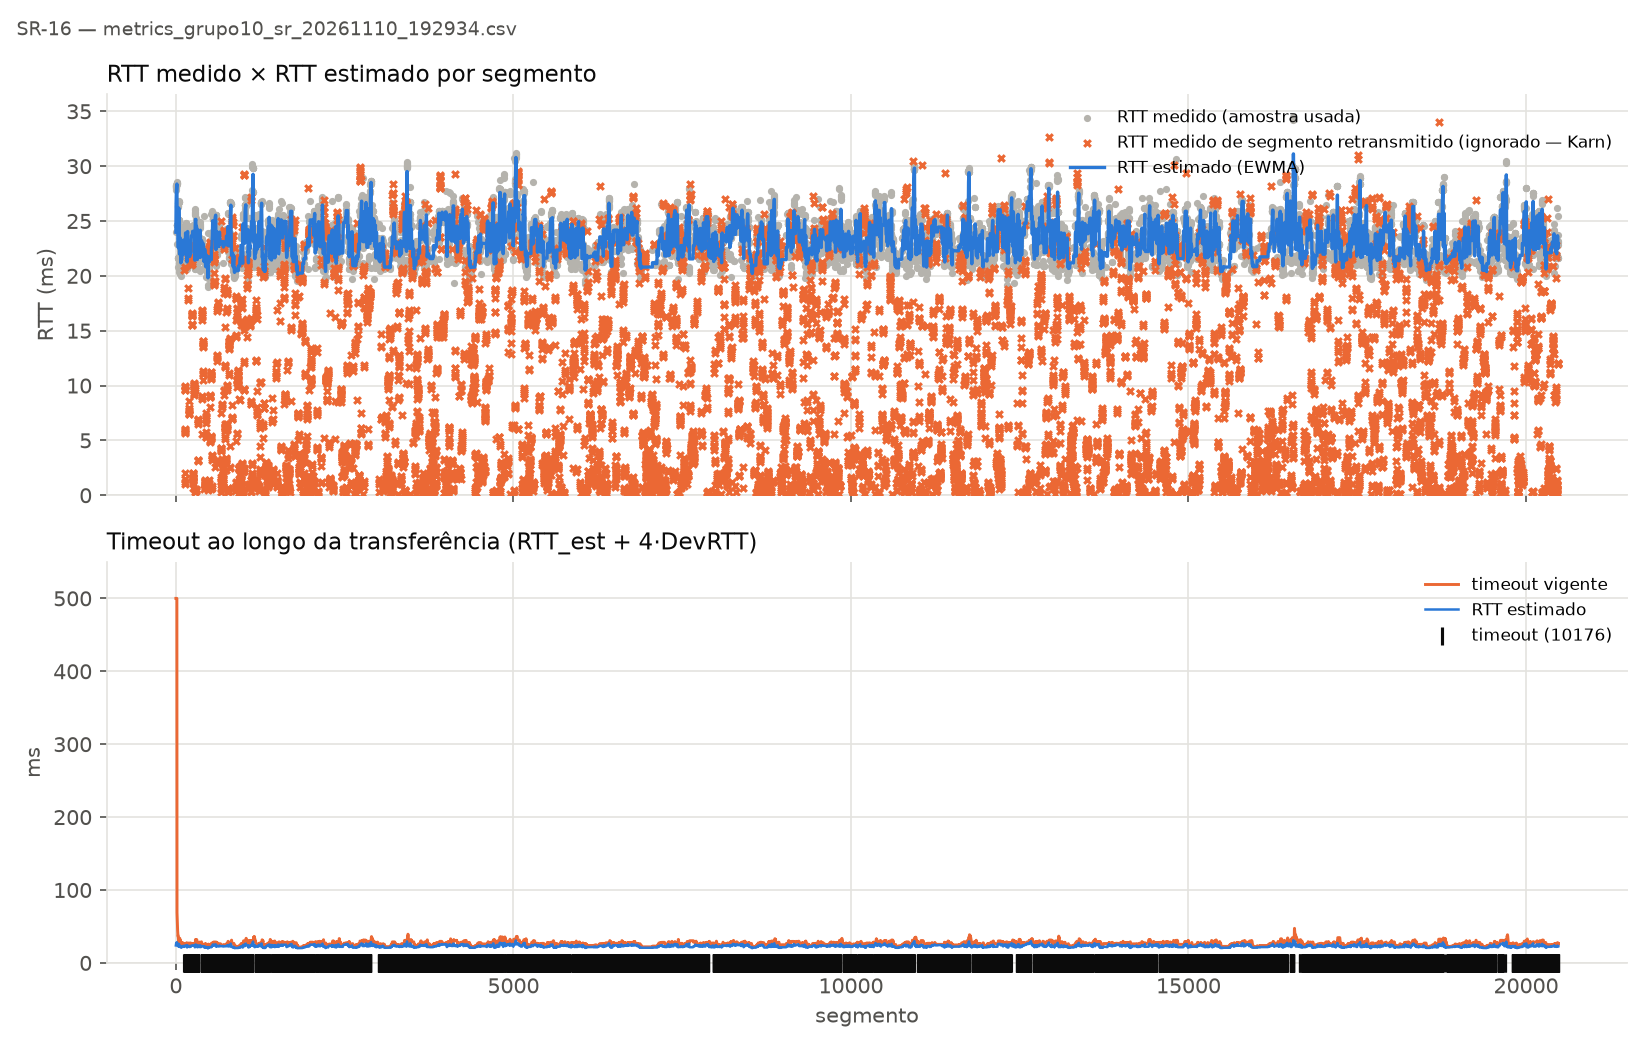
\includegraphics[width=0.95\textwidth]{figuras/rtt_sr16_large.png}
  \caption{SR-16 adaptativo, arquivo large, transferência inteira. Em cima: RTT estimado (EWMA)
  $\times$ RTT medido por segmento; em laranja, amostras de segmentos retransmitidos, ignoradas pelo
  estimador (Karn). Embaixo: timeout ao longo da transferência.}
  \label{fig:rtt}
\end{figure}

\begin{figure}[!htbp]
  \centering
  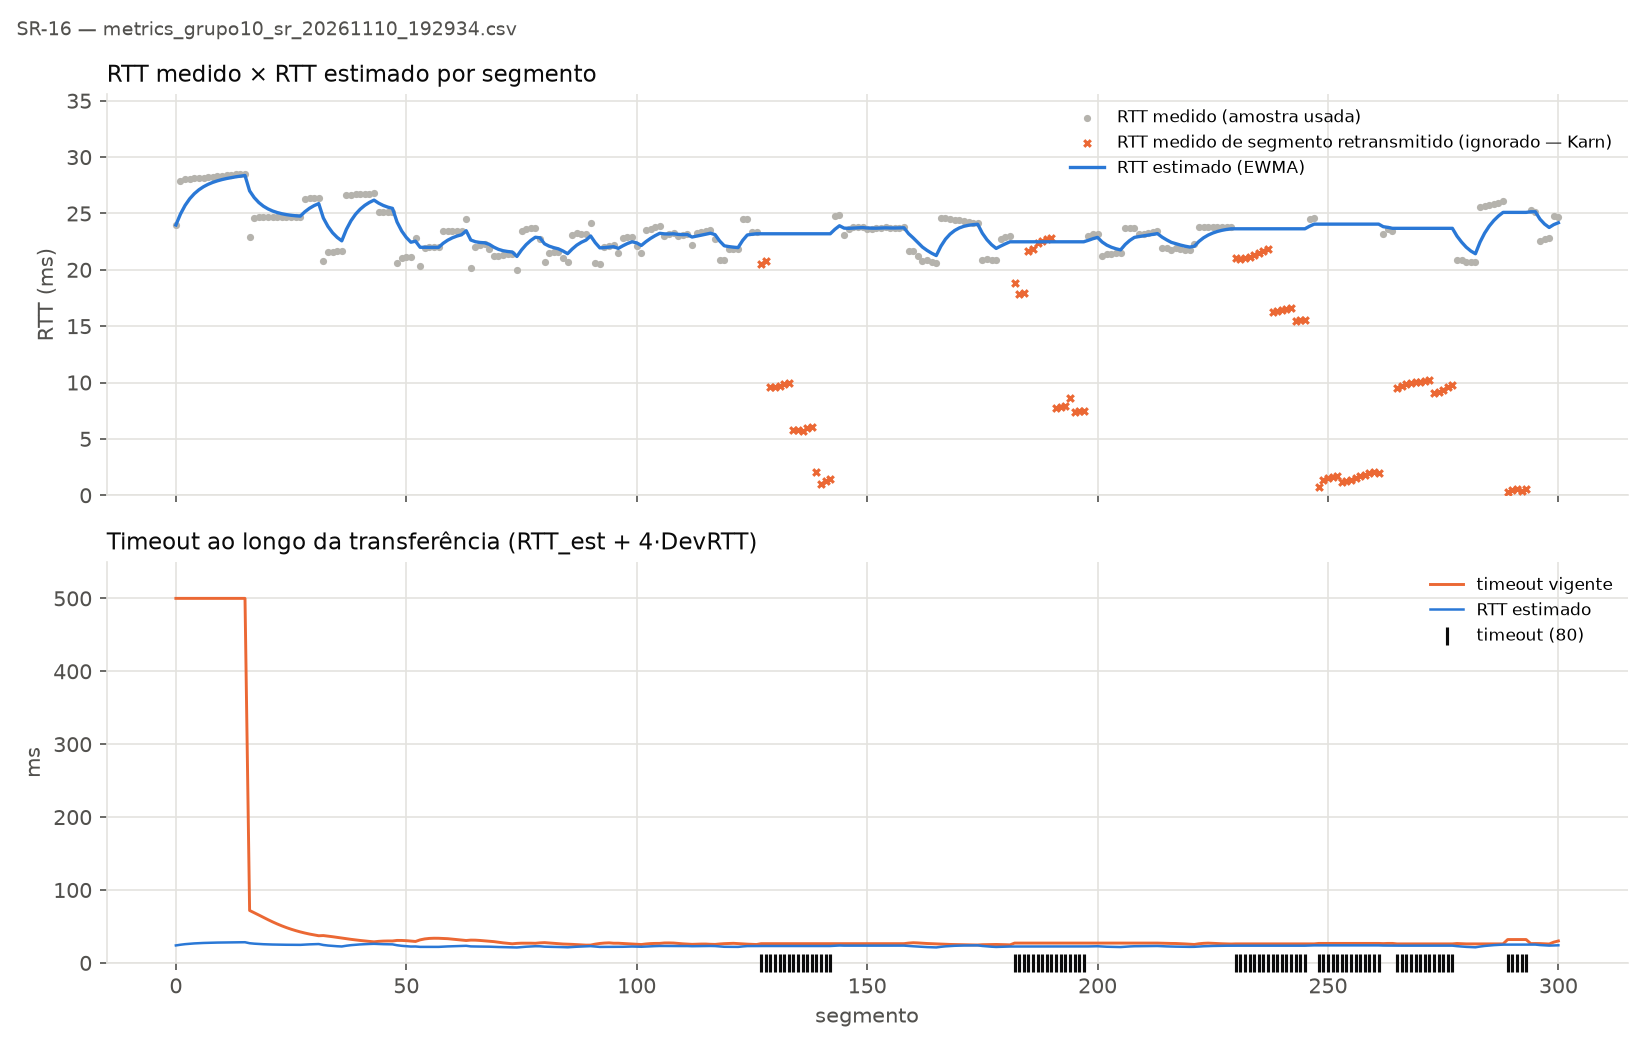
\includegraphics[width=0.95\textwidth]{figuras/rtt_sr16_large_0-300.png}
  \caption{Zoom nos 300 primeiros segmentos. Em cima: convergência do RTT estimado a partir da
  primeira amostra. Embaixo: o timeout cai de 500\,ms para $\sim$30\,ms e passa a acompanhar as
  variações do RTT.}
  \label{fig:rtt-zoom}
\end{figure}

%% ===========================================================================
\section{Comparação entre timeout fixo e adaptativo}\label{sec:comparacao}

\subsection{Método}

Comparamos o mesmo protocolo com timeout fixo (500\,ms) e adaptativo (com os $\alpha$ e $\beta$
escolhidos na Seção~\ref{sec:alfa-beta}) sob perda simulada de 5\,\% e 10\,\%, além do caso sem
perda como controle. Usamos GBN-16 e SR-16 (\cod{rtt\_adaptativo.py comparacao}), arquivo small,
\cod{-{}-seed 42} e as mesmas condições de rede: as execuções fixo e adaptativo de cada cenário
entraram na mesma rodada de experimentos, porque a rede varia de um dia para o outro
(Seção~\ref{sec:e2}). Os valores são médias de 2 repetições por cenário, todas com MD5 correto e
\cod{DONE ok=1}. Retransmissões espúrias são estimadas como retransmissões $-$ DATA descartados pela
simulação; no SR ela é quase exata com timeout fixo, mas subestima com o adaptativo (cópias duplicadas
de reenvios espúrios também são descartadas pela simulação e entram nos descartes), e no GBN inclui os
reenvios ``de carona'' do ``volta N'', então só é comparada entre fixo e adaptativo do mesmo protocolo.

Como referência, os valores com timeout fixo obtidos na Entrega 2 (uma execução, seed 42, outro dia)
foram: SR-16 com 5\,\% $\rightarrow$ 260,7\,kbps, 91 retransmissões, 32,2\,s; SR-16 com 10\,\%
$\rightarrow$ 153,7\,kbps, 220 retransmissões, 54,6\,s; GBN-16 com 5\,\% $\rightarrow$ 159,5\,kbps,
1\,512 retransmissões, 52,6\,s; GBN-16 com 10\,\% $\rightarrow$ 70,3\,kbps, 3\,562 retransmissões,
119,3\,s.

\subsection{Resultados}

\begin{table}[H]
\centering\footnotesize
\setlength{\tabcolsep}{3.5pt}
\caption{GBN-16 e SR-16, arquivo small, média de 2 execuções. Espúrias = retransmissões $-$ DATA
descartados pela simulação.}
\label{tab:fixo-adapt}
\begin{tabular}{@{}l r l rrrrrr@{}}
\toprule
\textbf{Protocolo} & \textbf{Perda} & \textbf{Timeout} & \hd{Retrans-\\missões} & \hd{Tempo\\(s)} &
\hd{Throughput\\(kbps)} & \hd{Descartes\\simulados} & \textbf{Espúrias} & \hd{Timeout\\médio (ms)}\\
\midrule
GBN-16 & 0\,\%  & fixo       & 16     & 5,76   & 1\,455,9 & 0   & 16     & 500\\
GBN-16 & 0\,\%  & adaptativo & 464    & 5,31   & 1\,578,9 & 0   & 464    & 48,9\\
GBN-16 & 5\,\%  & fixo       & 1\,512 & 55,73  & 150,5    & 156 & 1\,356 & 500\\
GBN-16 & 5\,\%  & adaptativo & 1\,926 & 12,37  & 678,9    & 172 & 1\,754 & 50,4\\
GBN-16 & 10\,\% & fixo       & 3\,598 & 123,71 & 67,8     & 536 & 3\,062 & 500\\
GBN-16 & 10\,\% & adaptativo & 4\,112 & 20,90  & 401,7    & 593 & 3\,519 & 48,6\\
\midrule
SR-16  & 0\,\%  & fixo       & 10     & 6,10   & 1\,411,8 & 0   & 10     & 500\\
SR-16  & 0\,\%  & adaptativo & 1\,007 & 4,83   & 1\,737,9 & 0   & 1\,007 & 39,3\\
SR-16  & 5\,\%  & fixo       & 105    & 33,77  & 248,5    & 91  & 14     & 500\\
SR-16  & 5\,\%  & adaptativo & 1\,466 & 6,92   & 1\,221,0 & 150 & 1\,316 & 35,6\\
SR-16  & 10\,\% & fixo       & 242    & 56,34  & 148,9    & 220 & 22     & 500\\
SR-16  & 10\,\% & adaptativo & 1\,343 & 8,46   & 991,2    & 326 & 1\,017 & 37,9\\
\bottomrule
\end{tabular}
\end{table}

\begin{figure}[H]
  \centering
  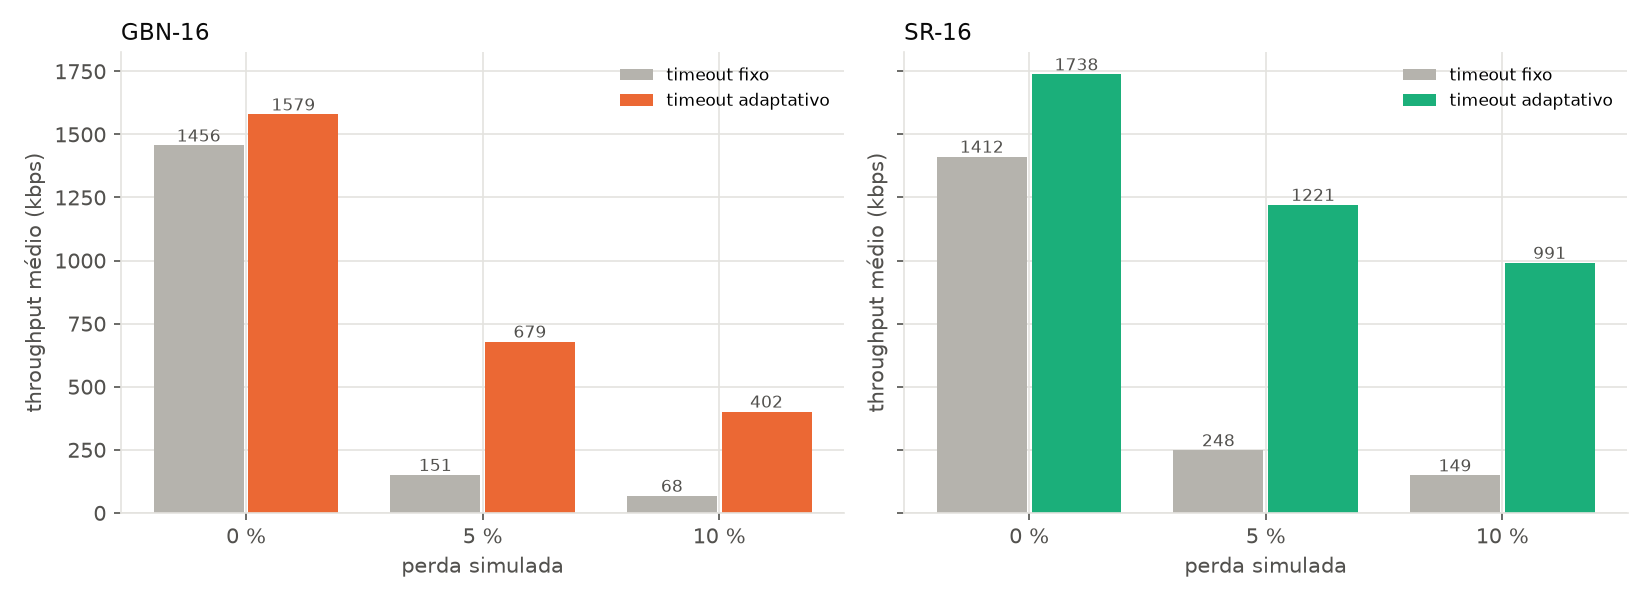
\includegraphics[width=0.95\textwidth]{figuras/fixo_vs_adaptativo.png}
  \caption{Throughput médio com timeout fixo e adaptativo, por perda simulada.}
  \label{fig:fixo-adapt}
\end{figure}

Com perda, o adaptativo cortou o tempo de transferência em 78\,\% a 85\,\%. No SR-16, o tempo caiu de
33,8\,s para 6,9\,s com 5\,\% de perda ($-80$\,\%) e de 56,3\,s para 8,5\,s com 10\,\% ($-85$\,\%), o
que multiplica a vazão por 4,9 e por 6,7. No GBN-16, a queda foi de 55,7\,s para 12,4\,s ($-78$\,\%)
e de 123,7\,s para 20,9\,s ($-83$\,\%), com vazão $\times 4{,}5$ e $\times 5{,}9$. Os resultados com
timeout fixo repetem os da Entrega 2 (por exemplo, GBN-16 com 5\,\%: 1\,512 retransmissões nas
duas). Mesmo adaptativo, o GBN-16 com 10\,\% (401,7\,kbps) ficou abaixo do SR-16 (991,2\,kbps).

Sem perda simulada, a diferença de tempo é pequena ($-21$\,\% no SR e $-8$\,\% no GBN), mas o número
de retransmissões sobe: o adaptativo fez 1\,007 retransmissões no SR e 464 no GBN, contra 10 e 16 com
o fixo. Com perda elas também aumentaram: no SR, de 105 para 1\,466 (5\,\%) e de 242 para 1\,343
(10\,\%); no GBN, 27\,\% e 14\,\% a mais. O adaptativo ganhou em tempo e perdeu em retransmissões,
compromisso discutido na Seção~\ref{sec:fixo-basta}.

\subsection{Quando o adaptativo vence e quando o fixo basta}\label{sec:fixo-basta}

Com perda, o adaptativo compensa muito; sem perda, o fixo basta, e o preço do adaptativo são as
retransmissões espúrias. Os pontos abaixo usam os números da Tabela~\ref{tab:fixo-adapt}.

\textbf{Onde o adaptativo tem mais vantagem: quando há perda.} Cada perda custa 500\,ms ao timeout
fixo, enquanto o timeout médio do adaptativo ficou em 36--50\,ms, de 10 a 14 vezes menor. A economia
cresce com a perda: 26,9\,s (SR) e 43,4\,s (GBN) com 5\,\%, e 47,9\,s (SR) e 102,8\,s (GBN) com
10\,\%. O efeito é maior no GBN, onde os timeouts se somam (Seção~\ref{sec:e2}): com 10\,\% de perda,
a vazão foi de 67,8 para 401,7\,kbps.

\textbf{Quando o fixo é suficiente: sem perda.} Sem perda simulada, fixo e adaptativo diferem só
pelas poucas perdas naturais da rede (10 retransmissões no SR e 16 no GBN com o fixo, cada uma
custando até 500\,ms), o que explica a diferença de 21\,\% e 8\,\% no tempo. Se a rede não perdesse
pacotes, ou se o tempo de recuperação não importasse, o fixo de 500\,ms seria suficiente, mais simples
e sem retransmissões desnecessárias.

\textbf{O preço: retransmissões espúrias.} Com perda zero, o adaptativo fez 1\,007 retransmissões no
SR (805 segmentos com timeout) e 464 no GBN, contra 10 e 16 com o fixo. O timeout médio (39\,ms no SR)
ficou muito perto do RTT médio (28\,ms), e os picos de RTT (de até $\sim$470\,ms na Entrega 1, além
do enfileiramento com janela 16) o ultrapassam. O mesmo aparece em todas as combinações da varredura.
No SR um espúrio custa um \cod{REQ} e um \cod{DATA} duplicado, que o cliente descarta; no GBN custa
até $N$ retransmissões de uma vez. Aqui isso não impediu o ganho de tempo, mas em uma rede com banda
disputada esses reenvios ocupariam o caminho e o servidor.

Uma explicação provável é o algoritmo de Karn sem backoff: as amostras de RTT longo são justamente as
que sofrem timeout espúrio e retransmissão, então são descartadas pelo estimador, e o RTO tende a
ficar baixo demais (Figura~\ref{fig:rtt}). Os testes naturais seriam dobrar o RTO após cada timeout,
como o TCP, ou subir o piso \cod{-{}-min-rto}, que já existe no cliente; testamos o piso na
Seção~\ref{sec:rto-min}.

Em resumo: neste ambiente (RTT de $\sim$28\,ms e perda alta), o adaptativo foi 4,5 a 6,7 vezes mais
rápido que o fixo e vale a pena quando há perda, preferencialmente no SR, que tolera melhor um RTO
agressivo (991,2\,kbps contra 401,7\,kbps do GBN com 10\,\%); sem perda, o fixo é suficiente.

\subsection{Teste do RTO mínimo}\label{sec:rto-min}

No arquivo large e sem perda, o efeito das espúrias passa a dominar: o SR-16 adaptativo fez 16\,749
retransmissões e ficou \emph{abaixo} do fixo (1\,690 contra 2\,067\,kbps, Tabela~\ref{tab:integrada}).
O TCP real evita isso com um RTO mínimo (200\,ms a 1\,s). Repetimos o SR-16 adaptativo com pisos de 50
e 100\,ms (\cod{-{}-min-rto}; uma execução por cenário, 20:13--20:15 de 10/11):

\begin{table}[H]
\centering\small
\caption{SR-16 adaptativo com RTO mínimo: throughput (kbps) / retransmissões.}
\label{tab:rto-min}
\begin{tabular}{@{}l cccc@{}}
\toprule
\textbf{Cenário} & \textbf{Sem piso (1\,ms)} & \textbf{Piso 50\,ms} & \textbf{Piso 100\,ms} & \textbf{Fixo 500\,ms}\\
\midrule
large, sem perda  & 1\,690 / 16\,749 & 2\,120 / 2\,183 & \textbf{2\,237 / 794} & 2\,067 / 13\\
small, sem perda  & 1\,738 / 1\,007  & \textbf{2\,190 / 162} & 2\,144 / 81 & 1\,412 / 10\\
small, 5\,\%      & \textbf{1\,221 / 1\,466} & 1\,201 / 317 & 824 / 175 & 249 / 105\\
small, 10\,\%     & \textbf{991 / 1\,343}  & 945 / 453 & 593 / 300 & 149 / 242\\
\bottomrule
\end{tabular}
\end{table}

O piso resolve o conflito entre os dois casos: sem perda, ele elimina a maior parte das espúrias
(16\,749 $\rightarrow$ 794 no large) e o adaptativo passa a superar o fixo; com perda, um piso alto
atrasa a recuperação das perdas reais (100\,ms: 593 contra 991\,kbps com 10\,\%). O piso de 50\,ms
ficou perto do melhor em todos os cenários (3\,\% acima do fixo no large e 55\,\% no small sem perda;
4,8$\times$ acima com 5\,\%).

%% ===========================================================================
\section{Análise Wireshark}\label{sec:wireshark}

Capturamos a transferência do SR-16 adaptativo com o arquivo large (10/11/2026, 19:28:45--19:29:34)
com o filtro \cod{udp and host 137.131.178.229}: 94\,948 pacotes, dos quais 37\,229 REQs
($=$ 20\,480 segmentos + 16\,749 retransmissões, exatamente o total do CSV).\\ Arquivo da captura: \repofile{entregas/entrega3/dados/large/captura_sr16_adaptativo_large.pcapng}{\cod{captura\_sr16\_adaptativo\_large.pcapng}}.

\begin{figure}[H]
  \centering
  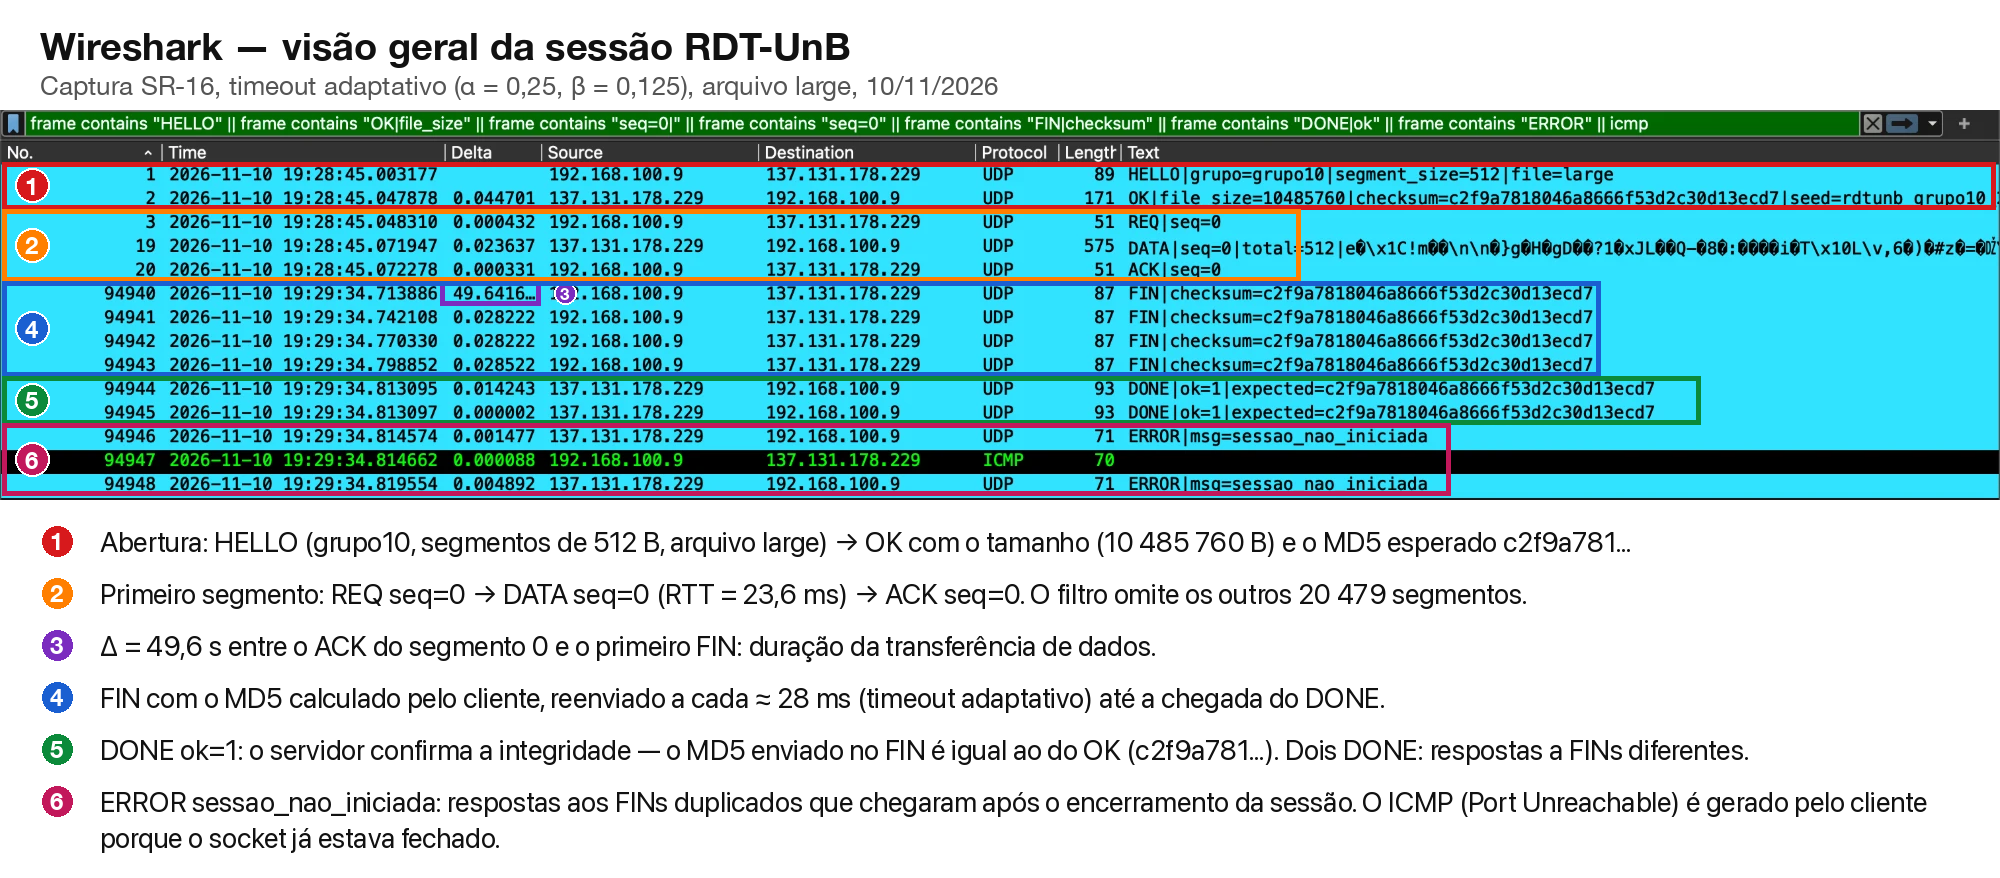
\includegraphics[width=\textwidth]{figuras/wireshark_visao_geral.png}
  \caption{Screenshot 1 --- visão geral da sessão: HELLO $\rightarrow$ OK $\rightarrow$
  REQ/DATA/ACK $\rightarrow$ FIN $\rightarrow$ DONE.}
  \label{fig:ws-geral}
\end{figure}

\begin{figure}[H]
  \centering
  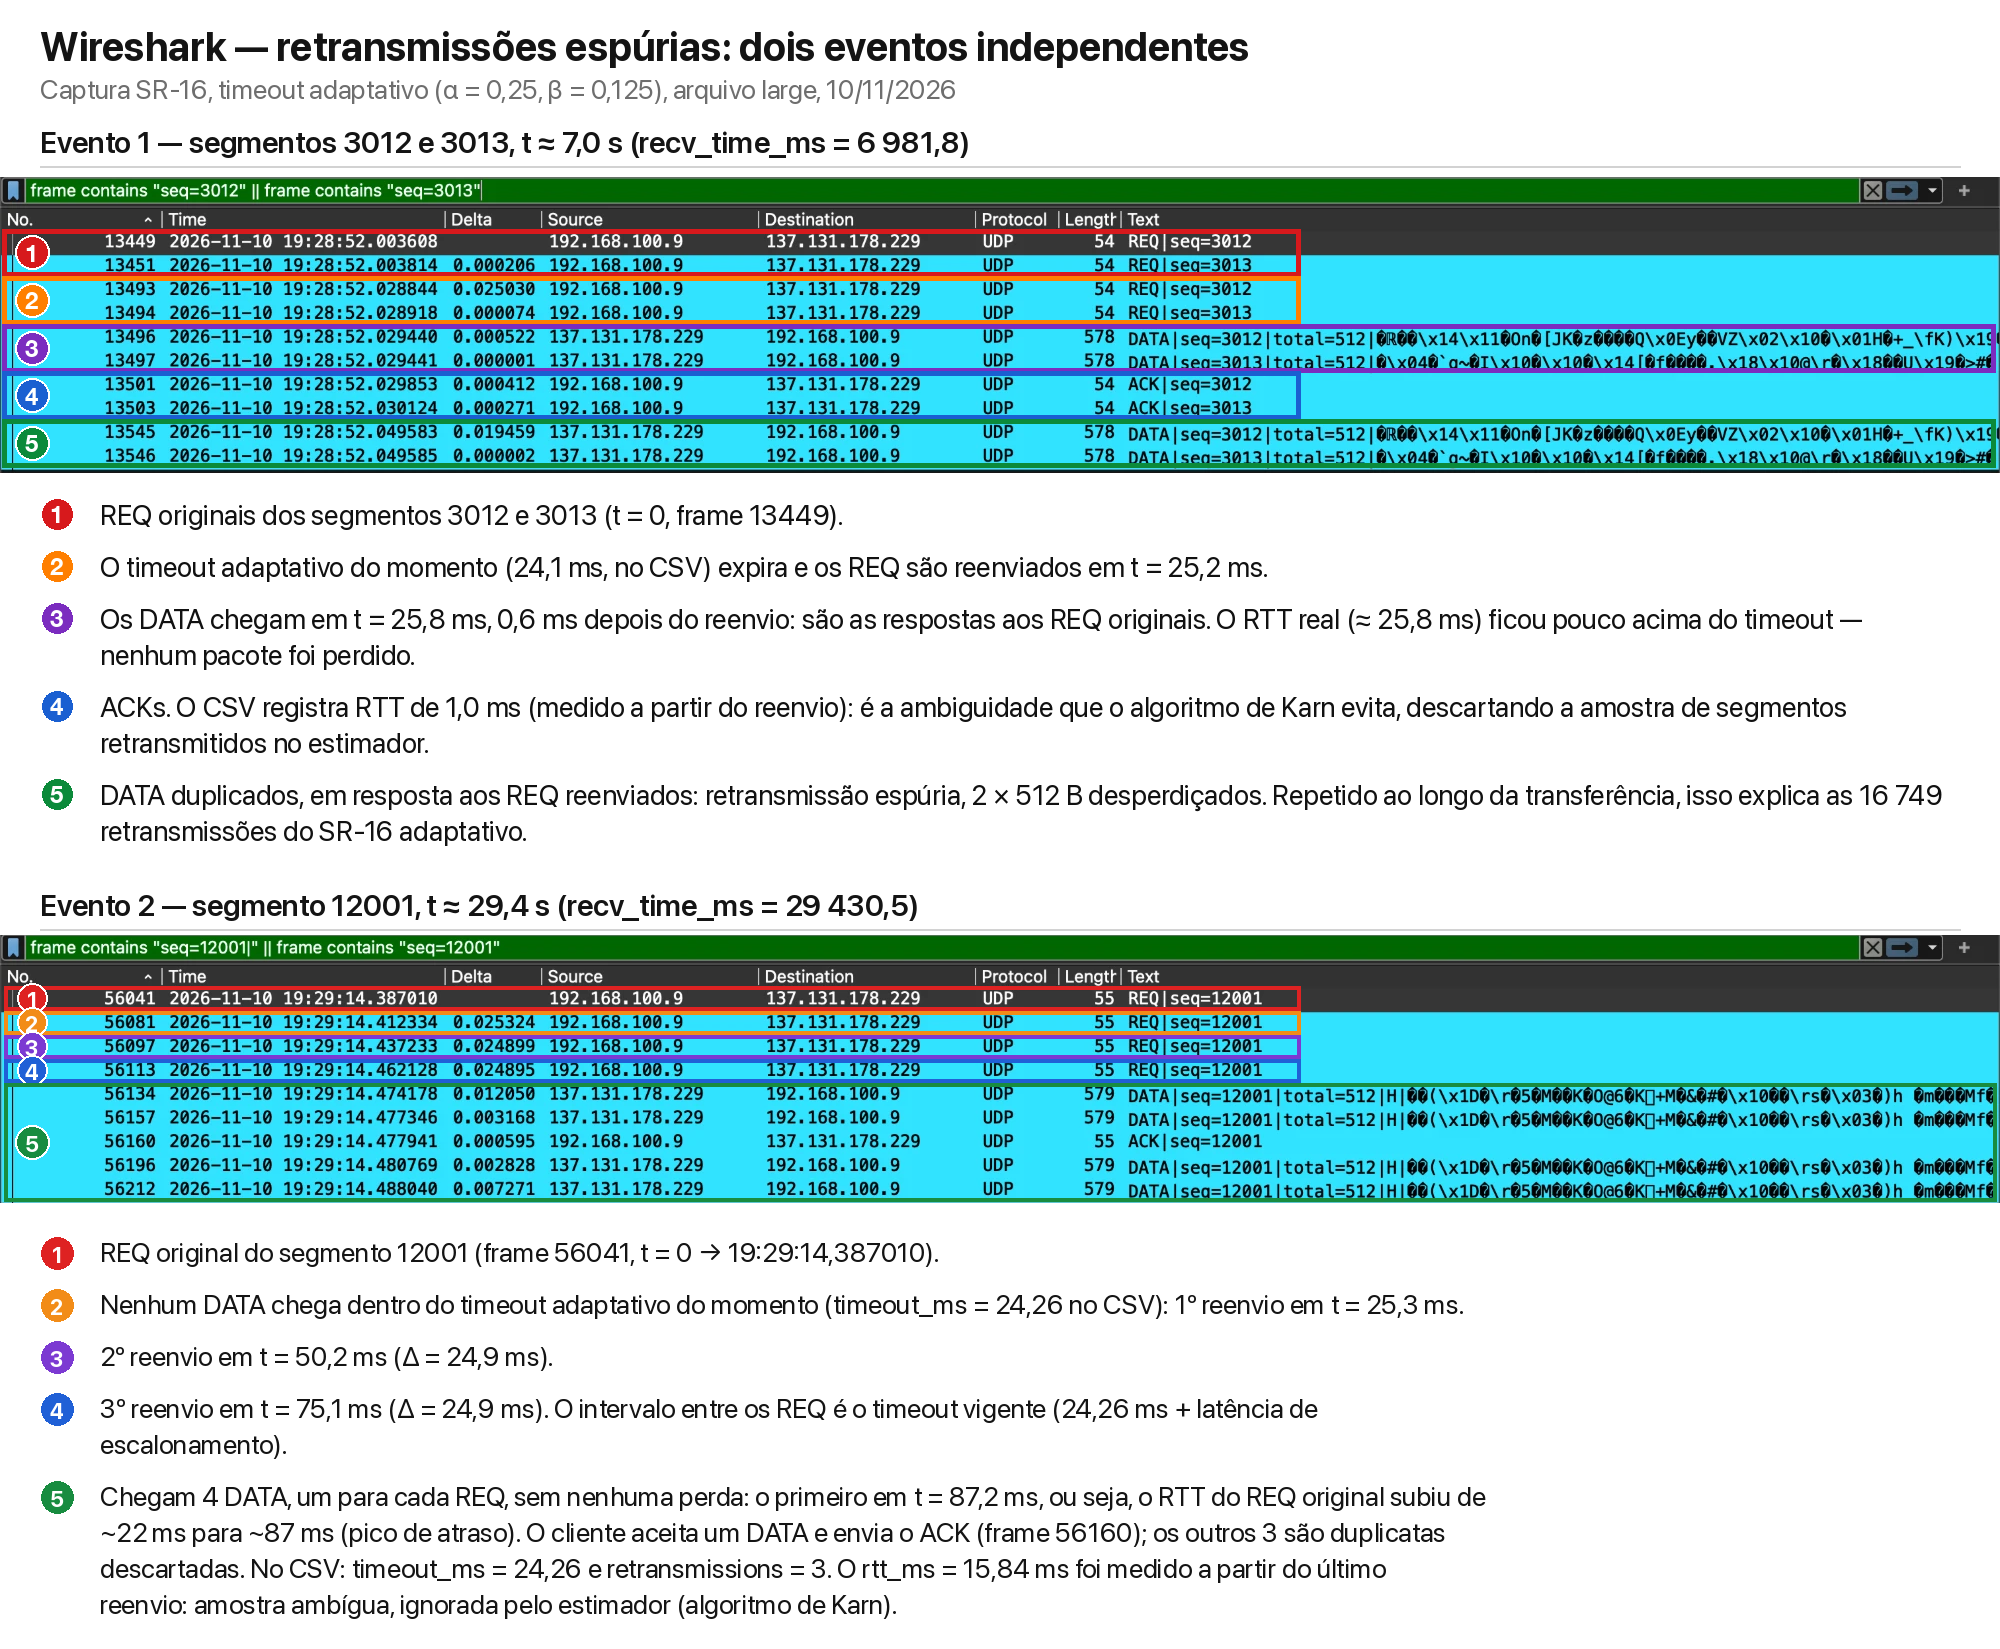
\includegraphics[width=\textwidth]{figuras/wireshark_retransmissoes.png}
  \caption{Screenshot 2 --- dois eventos de retransmissão independentes, em $t \approx 7{,}0$\,s
  (segmentos 3012 e 3013) e $t \approx 29{,}4$\,s (segmento 12001), com os tempos da coluna
  \cod{recv\_time\_ms} do CSV.}
  \label{fig:ws-retx}
\end{figure}

Nos dois eventos o REQ é reenviado depois de um intervalo próximo do timeout adaptativo vigente
(24,1\,ms e 24,26\,ms no CSV) e todos os DATA acabam chegando: são retransmissões
\textbf{espúrias}, causadas por picos de atraso e não por perda. No segmento 12001 o RTT do REQ
original foi de 87,2\,ms, o que gerou três reenvios e três DATA duplicados.

\begin{figure}[H]
  \centering
  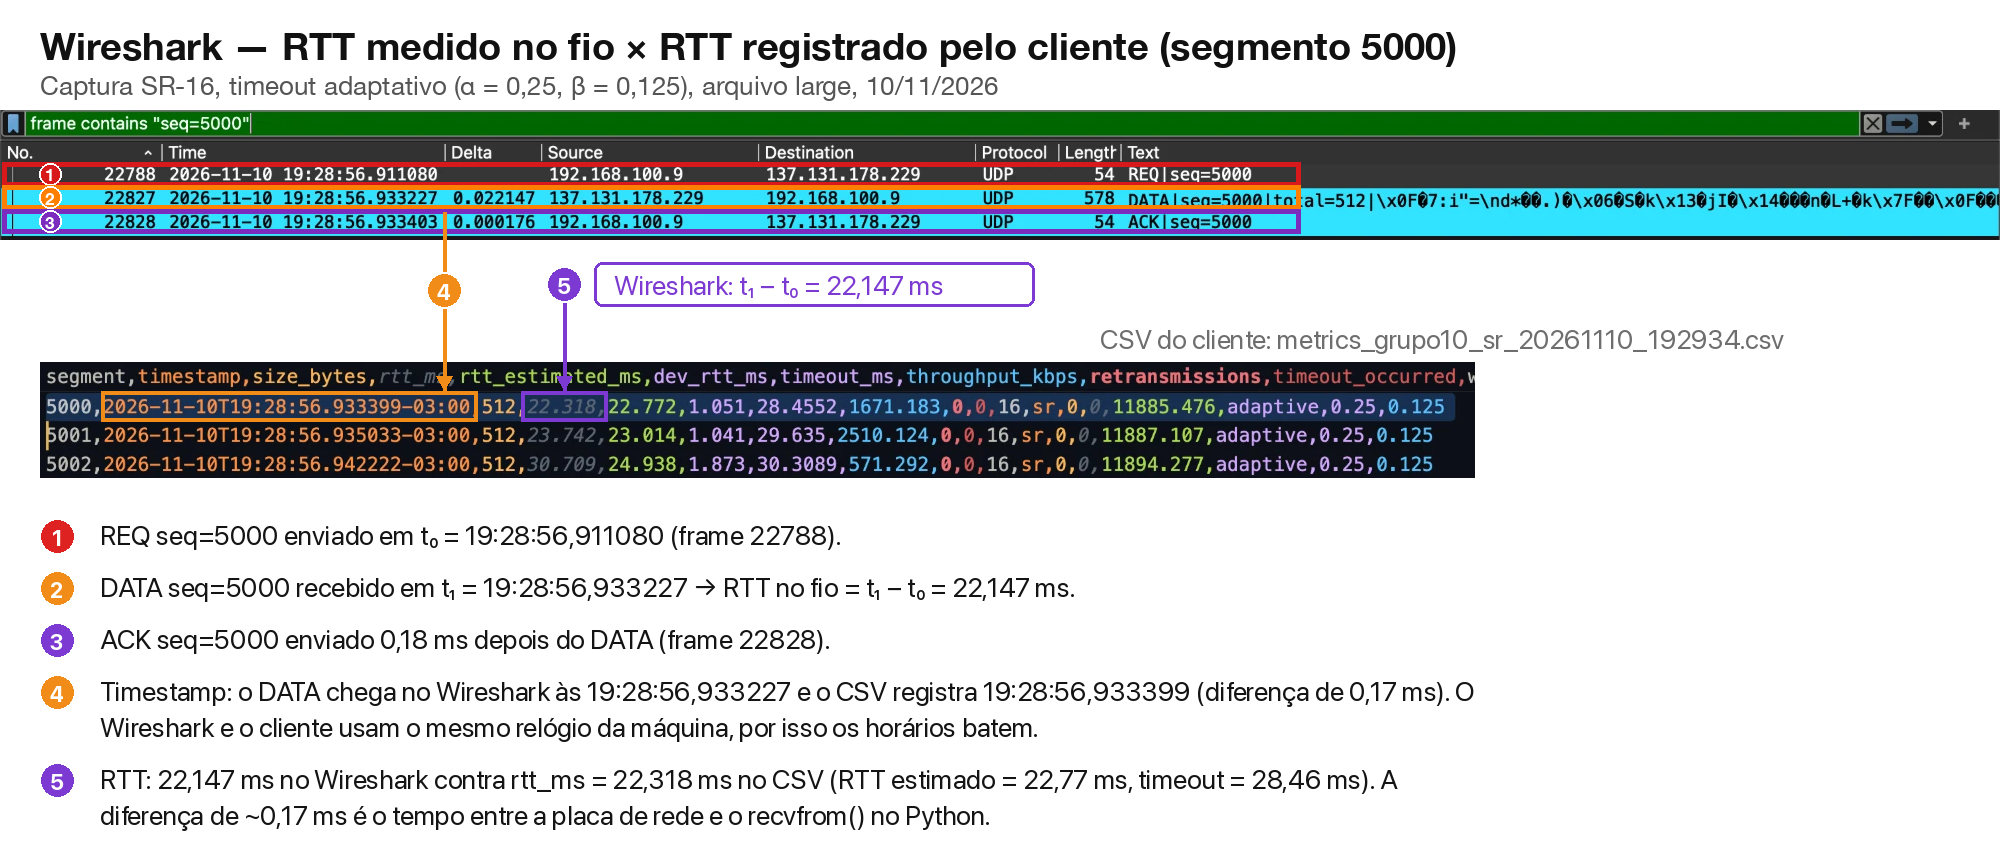
\includegraphics[width=\textwidth]{figuras/wireshark_rtt_seg5000_csv.png}
  \caption{Screenshot 3 --- correlação entre o Wireshark e a linha do segmento 5000 no CSV.}
  \label{fig:ws-csv}
\end{figure}

\textbf{RTT no Wireshark $\times$ RTT no CSV.} No segmento 5000, o RTT no fio foi 22,147\,ms e o do
CSV 22,318\,ms (diferença de 0,17\,ms); o timestamp do DATA é 19:28:56,933227 no Wireshark e
19:28:56,933399 no CSV. Os horários batem porque o Wireshark e o cliente usam o mesmo relógio da
máquina. Para não depender de um único segmento, extraímos do \cod{.pcapng} (com \cod{tshark}) o
tempo entre o REQ e o DATA de todos os segmentos com um único REQ e comparamos com o \cod{rtt\_ms}
do CSV:

\begin{table}[H]
\centering\small
\caption{RTT no fio (Wireshark) $\times$ RTT registrado pelo cliente, 10\,304 segmentos sem retransmissão.}
\label{tab:ws-rtt}
\begin{tabular}{@{}lrr@{}}
\toprule
& \textbf{Média (ms)} & \textbf{Mediana (ms)}\\
\midrule
Wireshark (DATA $-$ REQ)   & 22,51 & 22,39\\
CSV (\cod{rtt\_ms})        & 23,49 & 23,52\\
Diferença CSV $-$ Wireshark & 0,98 & 0,77\\
\bottomrule
\end{tabular}
\end{table}

Os valores são próximos: a diferença fica entre 0,19 e 2,43\,ms em 90\,\% dos segmentos e é
\emph{sempre positiva} (mínimo 0,08\,ms), como esperado. O Wireshark marca o instante em que o
pacote passa pela placa de rede; o cliente marca depois do \cod{recvfrom()} no Python. Com 16
segmentos em voo, os DATA chegam em rajadas e o cliente processa um de cada vez (ACK, linha do CSV,
novo REQ), então os últimos de cada rajada esperam alguns ms no buffer do socket. O segmento 5000
caiu num momento sem fila (0,17\,ms).

%% ===========================================================================
\section{Visão integrada --- comparação final de todos os protocolos}

Para comparar os protocolos nas mesmas condições de rede, rodamos todos com o arquivo large na mesma
janela de tempo (10/11/2026, 19:23--19:29), sem perda simulada. Todos terminaram com MD5
\cod{c2f9a7818046a8666f53d2c30d13ecd7} e \cod{DONE ok=1}.

\begin{table}[H]
\centering\small
\caption{Visão integrada: melhor cenário de cada protocolo, arquivo large (10\,MB), sem perda simulada.}
\label{tab:integrada}
\setlength{\tabcolsep}{4pt}
\begin{tabular}{@{}l r l rrr@{}}
\toprule
\textbf{Protocolo} & \textbf{Janela} & \textbf{Timeout} & \textbf{Throughput (kbps)} & \textbf{Retransmissões} & \textbf{Tempo total (s)}\\
\midrule
SAW & 1  & fixo       & 150,55   & 3       & 557,18\\
GBN & 16 & fixo       & 2\,014,30 & 96      & 41,65\\
GBN & 16 & adaptativo & 2\,092,78 & 4\,032   & 40,08\\
SR  & 16 & fixo       & 2\,067,29 & 13      & 40,58\\
SR  & 16 & adaptativo & 1\,690,49 & 16\,749  & 49,62\\
\midrule
SR  & 16 & adapt.\ + piso 100\,ms$^{*}$ & \textbf{2\,237,45} & 794 & \textbf{37,49}\\
\bottomrule
\multicolumn{6}{@{}l}{\footnotesize $^{*}$ Execução extra (20:15), Seção~3.1.}
\end{tabular}
\end{table}

\begin{figure}[H]
  \centering
  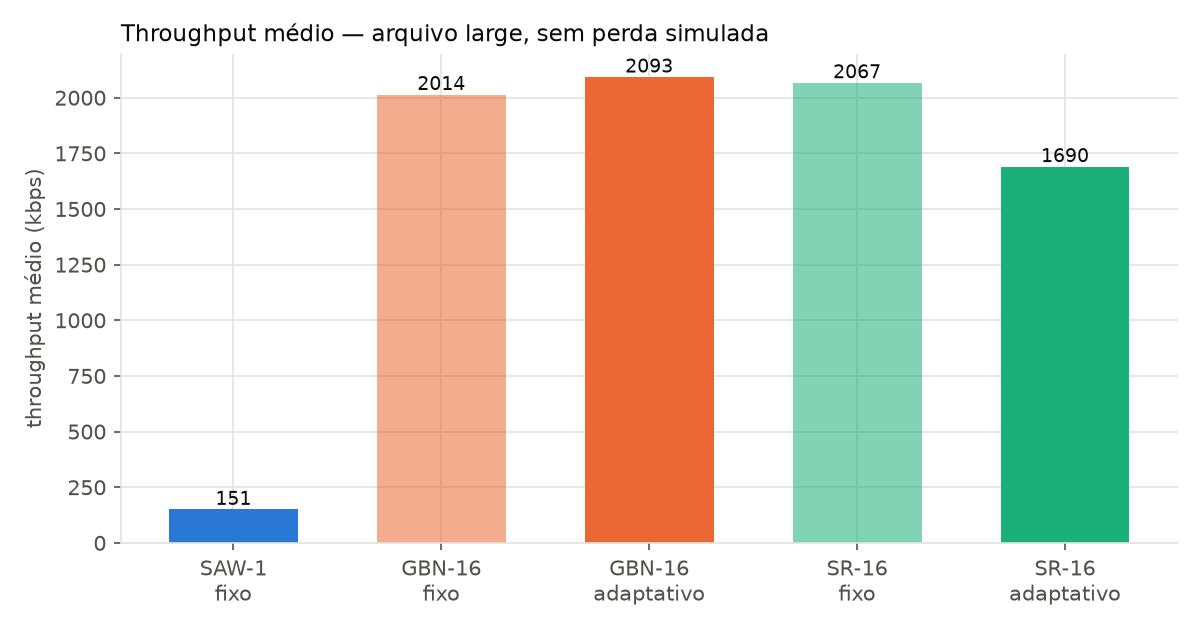
\includegraphics[width=0.85\textwidth]{figuras/comparacao_final.png}
  \caption{Throughput médio de todos os protocolos, arquivo large, sem perda simulada.}
  \label{fig:final}
\end{figure}

A tabela conta a história do projeto: a janela multiplicou a vazão por $\sim$14 (SAW 151 $\rightarrow$
GBN/SR $\sim$2\,000--2\,100\,kbps, tempo de 9 min para 40 s). O SAW da Entrega 1 com o mesmo
arquivo levou 965,9\,s (86,8\,kbps, 465 retransmissões naturais, 13/10/2026); a diferença para os
557\,s daqui é só a rede, mais estável no dia 10/11 (RTT médio de 35,6 contra 26,9\,ms e 3
retransmissões). Sem perda, GBN e SR ficam dentro de 4\,\% um do outro e o timeout adaptativo sem piso
não ajuda; os ganhos do SR e do timeout adaptativo aparecem com perda (Tabela~\ref{tab:todas-perda}).

\subsection{Todas as implementações com perda}

A Tabela~\ref{tab:todas-perda} junta as três entregas nos cenários com perda simulada (arquivo small,
\cod{-{}-seed 42}). As linhas de timeout fixo são da Entrega~2 (26/10/2026); as de timeout
adaptativo, da Entrega~3 (10/11/2026, média de 2 execuções).

\begin{table}[H]
\centering\small
\setlength{\tabcolsep}{5pt}
\caption{Todas as implementações, arquivo small: throughput (kbps) / retransmissões / tempo total (s).}
\label{tab:todas-perda}
\begin{tabular}{@{}l l ccc@{}}
\toprule
\textbf{Protocolo} & \textbf{Timeout} & \textbf{Sem perda} & \textbf{5\,\% de perda} & \textbf{10\,\% de perda}\\
\midrule
SAW-1  & fixo (E2)       & 167 / 0 / 50,2       & 88 / 91 / 95,0        & 52 / 220 / 161,3\\
GBN-16 & fixo (E2)       & 2\,026 / 0 / 4,1     & 159 / 1\,512 / 52,6   & 70 / 3\,562 / 119,3\\
GBN-16 & adaptativo (E3) & 1\,579 / 464 / 5,3   & 679 / 1\,926 / 12,4   & 402 / 4\,112 / 20,9\\
SR-16  & fixo (E2)       & 1\,901 / 0 / 4,4     & 261 / 91 / 32,2       & 154 / 220 / 54,6\\
SR-16  & adaptativo (E3) & 1\,738 / 1\,007 / 4,8 & \textbf{1\,221 / 1\,466 / 6,9} & \textbf{991 / 1\,343 / 8,5}\\
\bottomrule
\end{tabular}
\end{table}

\begin{itemize}
  \item \textbf{Sem perda, a janela é o que importa:} GBN-16 e SR-16 têm 11--12$\times$ o throughput
        do SAW, e o timeout quase não interfere. Na Entrega~2, a vazão cresceu com a janela
        (SAW 167 $\rightarrow$ $\sim$650 com $N=4$ $\rightarrow$ $\sim$1\,200 com $N=8$ $\rightarrow$
        $\sim$2\,000\,kbps com $N=16$).
  \item \textbf{Com perda e timeout fixo, o GBN quase não ganha do SAW} (10\,\%: 70 contra 52\,kbps):
        cada timeout reenvia a janela inteira (3\,562 retransmissões para as mesmas 220 perdas que o
        SR retransmite uma a uma) e trava a transferência por 500\,ms. O SR continua andando
        enquanto espera, e com $N=4/8/16$ foi de 84 para 110 e 154\,kbps; o GBN ficou em 64--70.
  \item \textbf{O timeout adaptativo multiplica o ganho do SR:} com 10\,\% de perda, o SR-16
        adaptativo (991\,kbps) mantém 57\,\% do próprio desempenho sem perda e 19$\times$ acima do
        SAW. O GBN também melhora (402\,kbps), mas continua limitado pelos reenvios em bloco.
  \item \textbf{Reprodutibilidade:} rodando de novo o timeout fixo em 10/11, com a mesma seed, os
        resultados com perda ficaram a menos de 6\,\% dos da Entrega~2 (GBN-16 10\,\%: 67,8 contra
        70,3\,kbps; SR-16 5\,\%: 248,5 contra 260,7\,kbps). Sem perda, a diferença é maior (SR-16:
        1\,412 contra 1\,901\,kbps), porque aí o resultado depende só da rede no dia.
\end{itemize}

%% ===========================================================================
\section{Conclusão}

\textbf{Qual protocolo teve melhor desempenho?} O \textbf{SR-16}. Sem perda, GBN-16 e SR-16 empatam
($\sim$2\,000--2\,100\,kbps, 14$\times$ o SAW). Com perda, o SR é claramente melhor: retransmite só o
segmento perdido, enquanto o GBN reenvia a janela inteira (com 10\,\% de perda e timeout adaptativo,
SR-16 991\,kbps contra GBN-16 402\,kbps; 1\,343 contra 4\,112 retransmissões). O melhor resultado
absoluto no arquivo large foi o SR-16 adaptativo com piso de 100\,ms (2\,237\,kbps, 37,5\,s).

\textbf{O RTT adaptativo valeu a complexidade?} Sim, mas com uma condição. Com perda, foi a mudança
de maior impacto do projeto: 4,5--6,7$\times$ mais throughput que o fixo (Tabela~\ref{tab:fixo-adapt}),
porque cada perda passou a custar $\sim$1--2 RTTs em vez de 500\,ms. Sem perda e com RTT estável,
a fórmula pura do livro deixou o timeout colado no RTT e piorou o SR no arquivo large (1\,690 contra
2\,067\,kbps). A complexidade só compensa por completo junto com um RTO mínimo: com piso de 50\,ms o
adaptativo ficou perto do melhor em todos os cenários testados (Tabela~\ref{tab:rto-min}).

\textbf{O que faríamos diferente.}
\begin{itemize}
  \item Registrar no CSV o RTT medido a partir do \emph{primeiro} REQ, além do último, para não
        depender só de Karn para tratar a ambiguidade.
  \item Rodar os experimentos com antecedência, como pegamos os dados somente do último dia, 
        pode ser que tenhamos perdido uma rede mais estável. Na primeira rodada do
        arquivo large (10/11, 18:32--18:47) pegamos a rede degradada (o SAW levou 1\,114\,s, com
        772 retransmissões naturais, contra 557\,s e 3 retransmissões na rodada das 19:23)
        e precisou ser refeita.\end{itemize}

%% ===========================================================================
\appendix
\section*{Anexo A --- CSVs e demais arquivos (links)}

Todos os arquivos estão no repositório público
\href{\repobase/tree/\reporef}{\cod{github.com/annalujansen/tr2-rdt-unb}} (tag \cod{entrega3}).
Os CSVs por segmento seguem o padrão
\cod{metrics\_grupo10\_\textless protocolo\textgreater\_\textless AAAAMMDD\_HHMMSS\textgreater.csv},
um por execução, numa pasta por cenário; cada conjunto tem um \cod{resumo*.csv} com uma linha por
execução (tempo, RTT, throughput, retransmissões, MD5).
\begin{itemize}
  \item \textbf{Entrega 1} --- \repodir{entregas/entrega1/dados}{\cod{entrega1/dados/}}: SAW com small,
        medium e large (13/10/2026).
  \item \textbf{Entrega 2} --- \repodir{entregas/entrega2/dados}{\cod{entrega2/dados/}}: 21 cenários
        (SAW, GBN e SR; janelas 4, 8 e 16; perdas 0, 5 e 10\,\%) e
        \repofile{entregas/entrega2/dados/tabela_comparativa.csv}{\cod{tabela\_comparativa.csv}}.
  \item \textbf{Entrega 3} --- \repodir{entregas/entrega3/dados}{\cod{entrega3/dados/}}:
  \begin{itemize}
    \item \repodir{entregas/entrega3/dados/varredura}{\cod{varredura/}} --- varredura $\alpha \times \beta$ (Seção~2.2);
    \item \repodir{entregas/entrega3/dados/comparacao}{\cod{comparacao/}} --- timeout fixo $\times$ adaptativo (Seção~3);
    \item \repodir{entregas/entrega3/dados/rto_minimo}{\cod{rto\_minimo/}} --- RTO mínimo (Seção~3.1);
    \item \repodir{entregas/entrega3/dados/large}{\cod{large/}} --- arquivo large, tabela integrada e captura (Seções~4 e~5);
    \item \repodir{entregas/entrega3/dados/large_rodada1}{\cod{large\_rodada1/}} --- primeira rodada do large, com a rede degradada.
  \end{itemize}
\end{itemize}
CSV das Figuras~\ref{fig:rtt}--\ref{fig:ws-csv}:
\repofile{entregas/entrega3/dados/large/large_sr_w16_loss0_adapt_a0.25_b0.125/metrics_grupo10_sr_20261110_192934.csv}{\cod{metrics\_grupo10\_sr\_20261110\_192934.csv}}.

\section*{Anexo B --- Checksum MD5 dos arquivos recebidos}

O cliente calcula o MD5 do arquivo remontado e o envia no \cod{FIN}; o servidor compara com o MD5
informado no \cod{OK} e responde \cod{DONE|ok=1}. Em todas as execuções, \cod{md5\_ok = 1} e
\cod{done\_ok = 1}. O conteúdo gerado pelo servidor mudou entre as entregas (por isso o MD5 do
mesmo arquivo difere), mas em cada sessão o MD5 recebido bateu com o informado no \cod{OK}
(Figura~\ref{fig:ws-geral}).

\begin{table}[H]
\centering\footnotesize
\setlength{\tabcolsep}{4pt}
\begin{tabular}{@{}c l l l l@{}}
\toprule
\textbf{Entrega} & \textbf{Protocolos} & \textbf{Timeout} & \textbf{Arquivo} & \textbf{MD5 recebido (= esperado)}\\
\midrule
1 & SAW & fixo & small  & \texttt{f989450f6ca695013ceb6bd3a5f6417c}\\
1 & SAW & fixo & medium & \texttt{2593bb16a3f52e31a7b8773450e8da8b}\\
1 & SAW & fixo & large  & \texttt{5623bc385a7b296e6c57d99290c03c0f}\\
2 & SAW, GBN-4/8/16, SR-4/8/16 & fixo & small  & \texttt{f989450f6ca695013ceb6bd3a5f6417c}\\
3 & GBN-16, SR-16 & fixo, adapt. & small  & \texttt{669af092d18cc3f9a060e9d1fb630d64}\\
3 & SAW, GBN-16, SR-16 & fixo e/ou adapt. & large  & \texttt{c2f9a7818046a8666f53d2c30d13ecd7}\\
\bottomrule
\end{tabular}
\end{table}

\end{document}
